\section{Bottom-Up Approach}
\label{sec:bottomup}

\subsection{HMMs}

Once we had created our methodology for splitting up time series using change-
point detection, we decided to test it against a more standard,
baseline technique. For this approach, we used the Hidden Markov Model to take
advantage of the sequential nature of our data. An HMM is a temporal graphical model
that contains a set of hidden states $H = \{H_0,H_1, \ldots, H_w\}$ as well as a set of
observed states $O = \{O_1,O_2, \ldots, O_w\}$ (Figure \ref{fig:hmm}). An index
of either type of state represents a point in time, such that if there exists
two indices $i$ and $j$ where $i < j$, $i$ is thought of as having happened
before $j$. Each hidden state in the model has one of a discrete set of values associated
with it drawn from $X=\{X_1,X_2, \ldots, X_{\ell}\}$, and each observed state has one
of a discrete set of values associated with it drawn from $Y=\{Y_1,Y_2, \ldots, Y_m\}$.
The values of the hidden states are unknown, and the values of the observable
states are known.
It is also assumed that, as indicated by Figure \ref{fig:hmm}, the
value of an observable state $O_i$ is dependent on the corresponding
hidden state $H_i$, and that the value of any hidden state $H_i$ is dependent only on
its immediate predecessor $H_{i-1}$.

Furthermore, the dependencies between hidden states and their followers are
assumed to be described by a stationary stochastic process known as the
\emph{transition model}, \mbox{$T: X^2 \rightarrow [0,1]$}. The dependencies
between a hidden state and its adjacent observable state are assumed to be part
of a separate but also stationary stochastic process known as the
\emph{observation model}, $S: X \times Y \rightarrow [0,1]$. In other words, both
models can be thought of as a function of two values, that output the
probability of a change from the first value to the second via a dependency
arc in the HMM. The usual approach to estimating $T$ and $S$ given only
$O$ is a flavor of expectation maximation known as the Baum-Welch algorithm,
which is useful for finding $\hat{T}$ and $\hat{S}$ that are locally maximally
likely. However, suppose a \emph{training HMM} $\langle H_{tr},O_{tr} \rangle$
with the same model parameters is given, and the values of all of its hidden states as well as its
observable states are known. $T$ and $S$ are then approximated by the
following global maximum likelihood estimators:

\[
\hat{T}(X_i,X_j) = \frac{|\{H_k \in H_{tr} \; | \; H_k=X_i \; \text{and} \; H_{k+1}=X_j\}|} {|\{H_k \in H_{tr} \; | \; H_k=X_i\}|}
\]

\[
\hat{S}(X_i,Y_j) = \frac{|\{H_k \in H \; | \; H_k=X_i \; \text{and} \; O_k=Y_j\}|} {|\{H_k \in H \; | \; H_k=X_i\}|}
\]

\begin{figure}
 \centering
 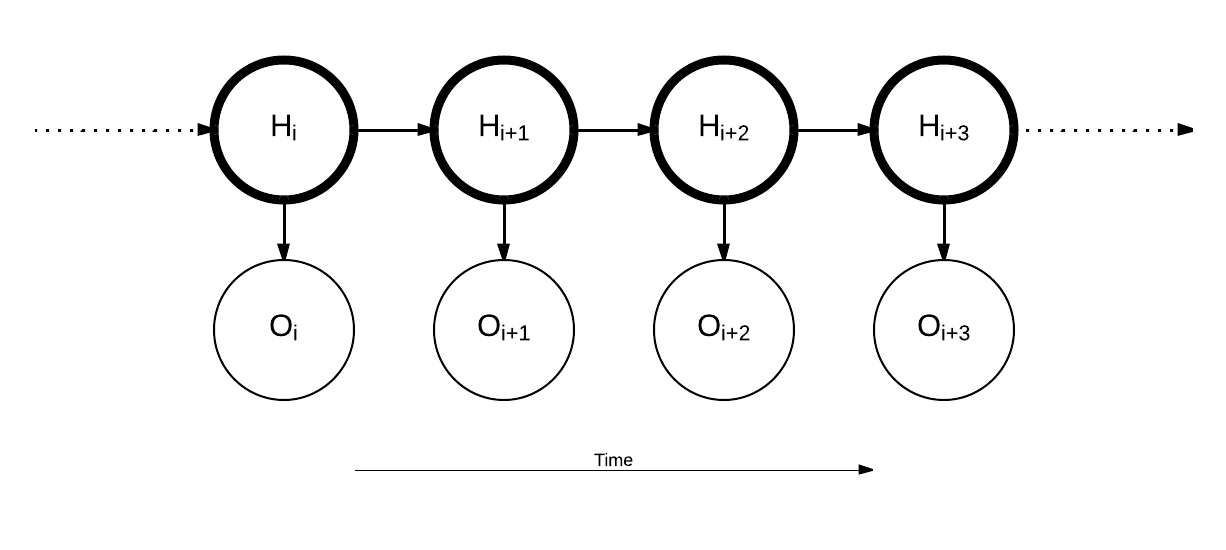
\includegraphics[scale=0.3]{hmm.png}
 \caption{Visual Interpretation of an HMM}
 \label{fig:hmm}
\end{figure}

Finally, if all of the values of $O$ are known, and we are given
a $\hat{T}$ and an $\hat{S}$ estimated from a training HMM, then the goal we are interested in
is to use that information (along with the model assumptions)
to find the most likely values for each state in $H$. There
exists a polynomial-time dynamic programming solution to this problem known as
the Viterbi algorithm. \cite{russell10}

\subsection{Experimental Setup}

For our experiments we began by splitting each time series into small non-overlapping windows. Within a
given experiment the window size was fixed, but across different experiments we
tested window sizes of length $\{1,2, \ldots ,20\}$. Once the time series were
split they were featurized. Classification
models were built with training data,
and tuned (in the case of the svm and neural net models) using validation data,
in the same way that has already been described previously in this chapter.

Unlike the change-point detection experiments, this experiment required
that the data be split into 4 equal parts: training (classifier), validation,
training (HMM), and testing) rather than 3. 
Here we formulated the problem of making predictions on the testing set in terms
of an HMM, first by treating the second training set as a training HMM. Each
window of the second training set was treated as a time index ${1,2, \ldots, n}$.
In our datasets we
let $H$ be the ground truth activity classes of the windows, and $O$ be the
predicted activity classes of the windows. We used the precedure above to
calculate $\hat{T}$ and $\hat{S}$, and assumed that these estimates held for
the testing set as well as the second training set. We then used the
tuned base classifier to predict on the testing set, giving us $O$. Finally,
we used $O$, $\hat{T}$, and $\hat{S}$ to run the Viterbi algorithm on the
testing set and predict the ground truth activity classes $H$.
